\documentclass[tikz,border=8pt]{standalone}
\usetikzlibrary{arrows.meta}
\begin{document}
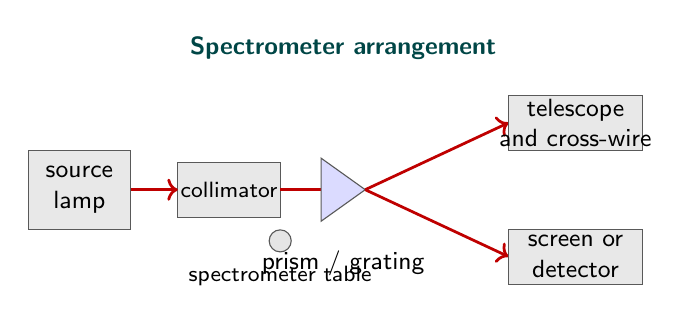
\begin{tikzpicture}[font=\sffamily\small]
\node[font=\sffamily\bfseries\small,text=teal!55!black] at (0,3.3) {Spectrometer arrangement};
\draw[fill=gray!18,draw=black!65] (-4,1.0) rectangle (-2.7,2.0);
\node[align=center] at (-3.35,1.5) {source\\lamp};
\draw[fill=gray!18,draw=black!65] (-2.1,1.15) rectangle (-.8,1.85);
\node[align=center,font=\sffamily\footnotesize] at (-1.45,1.5) {collimator};
\draw[->,red!75!black,line width=1pt] (-2.7,1.5)--(-2.1,1.5);
\draw[->,red!75!black,line width=1pt] (-.8,1.5)--(-.05,1.5);
\draw[fill=blue!14,draw=black!65] (-.28,1.1)--(.28,1.5)--(-.28,1.9)--cycle;
\node[below=.2cm] at (0,1.05) {prism / grating};
\draw[->,red!75!black,line width=1pt] (.28,1.5)--(2.1,2.35);
\draw[fill=gray!18,draw=black!65] (2.1,2.0) rectangle (3.8,2.7);
\node[align=center] at (2.95,2.35) {telescope\\and cross-wire};
\draw[->,red!75!black,line width=1pt] (.28,1.5)--(2.1,.65);
\draw[fill=gray!18,draw=black!65] (2.1,.3) rectangle (3.8,1.0);
\node[align=center] at (2.95,.65) {screen or\\detector};
\draw[fill=black!10,draw=black!65] (-.8,.85) circle (.14);
\node[below=.1cm,font=\sffamily\footnotesize] at (-.8,.75) {spectrometer table};
\end{tikzpicture}
\end{document}
